\documentclass[11pt,a4paper]{article}
\usepackage[T1]{fontenc}
\usepackage{lmodern}
\usepackage{amsmath,amssymb,graphicx,booktabs,array,tabularx,multirow}
\usepackage[margin=1in]{geometry}
\usepackage[numbers,sort&compress]{natbib}
\usepackage{xcolor}
\usepackage[hidelinks]{hyperref}
\usepackage{microtype,caption,placeins}
\usepackage{tikz}
\usetikzlibrary{positioning,arrows.meta}
\hypersetup{pdftitle={Known-answer screening for industrial fault diagnosis with large language models: prospective evaluation and failure analysis},pdfauthor={Song Ouyang, Xin Lu, Yan Yu}}
\captionsetup{font=small,labelfont=bf}
\setlength{\emergencystretch}{2em}
\clubpenalty=10000
\widowpenalty=10000
\renewcommand{\topfraction}{0.9}
\renewcommand{\textfraction}{0.08}
\renewcommand{\floatpagefraction}{0.7}
\definecolor{cblue}{HTML}{2A78D6}
\definecolor{corange}{HTML}{EB6834}
\definecolor{caqua}{HTML}{1BAF7A}
\definecolor{cink}{HTML}{52514E}
\newcommand{\todo}[1]{\textcolor{red}{[TODO: #1]}}

\title{Known-answer screening for industrial fault diagnosis with large language models: prospective evaluation and failure analysis}
\author{Song Ouyang$^{a,}$\thanks{Corresponding author. E-mail: ouyangsong8@gmail.com. ORCID: 0009-0003-0441-6337.}, Xin Lu$^{b}$, Yan Yu$^{c}$\\[4pt]
\small $^{a}$Independent Researcher, Chengdu, Sichuan, China\\
\small $^{b}$Independent Researcher, Wuhan 430014, China\\
\small $^{c}$School of Artificial Intelligence and Law, Southwest University of Political Science and Law,\\ \small Chongqing 401120, China}
\date{}

\begin{document}
\maketitle

\begin{abstract}
Known-answer reference records may help screen unreliable responses when a large language model diagnoses several industrial records in one request. We evaluated a fixed screen requiring at least eight of nine reference diagnoses to be correct, with their labels withheld from the model and at most three attempts per decision window. In a locally frozen 27-call hydraulic experiment, screening reduced accepted-label error from 35.2\% to 2.4\% at 77.8\% coverage. A post hoc control rejecting near-monolabel outputs achieved identical window results, leaving the incremental value of reference answers unresolved. We then fixed both rules before 18 further calls using new focal and reference blocks in a later service period. Across six windows, known-answer screening released 100 correct and eight incorrect labels out of 108 planned decisions, compared with 88 correct and 20 incorrect for both the first call and concentration control. Coverage was 100\%; offline replay required 1.5 calls per window rather than one. Three-call voting yielded 84 correct labels. Earlier repeated-call studies on two simulated and two measured systems characterize persistent errors and input dependence. The follow-up supports a specific benefit beyond concentration detection, while eight residual errors on two repeatedly assessed cycles show incomplete protection. Reused records, one hydraulic rig and jointly changed source panels, service period and client version limit generalization.
\end{abstract}
\noindent\textbf{Keywords:} fault diagnosis; large language models; repeatability; selective prediction; known-answer screening

\section{Introduction}
Data-driven fault diagnosis has moved from hand-crafted features to deep networks trained on large labelled datasets \citep{lei2020applications,zhao2019deep}. Large language models (LLMs) add text-based approaches to diagnosis, including task-specific fine-tuning \citep{qaid2026explainable,zheng2024empirical} and broader foundation-model workflows for prognostics and health management \citep{li2024chatgptphm}. Here, we examine a general-purpose service that receives measurements as text and returns diagnostic labels without task-specific training. The appeal for industrial users is clear. A single interface can serve many assets, domain knowledge about sensors and failure modes can be expressed in words, and the model can be queried by engineers who do not maintain a classifier.

This convenience depends on a serialization layer that is easy to overlook. Each measured value has to be written next to a channel identifier, a name and a unit, and several observations are often packed into one request to reduce cost \citep{cheng2023batch,lin2024batchprompt}. Two practical errors follow. A conversion script can attach the description of one sensor to the value of another while leaving every number in place. Separately, a correctly serialized observation can receive a different label because the other records in the request, or its position among them, have changed. The first error alters the physical meaning of the input; the second leaves the target record intact. Both are routine engineering risks, and both are invisible to an evaluation that reports only accuracy on clean inputs.

Evaluating these errors is complicated by a third factor. Commercial LLM services do not always return the same answer to the same request, even at nominally deterministic settings \citep{ouyang2025nondeterminism,atil2025nondeterminism}. When an intervention is tested with one call per condition, any label change can reflect the intervention, the service's call-to-call variation or a change in the service between calls. Related work on tabular and batched LLM inference has shown sensitivity to feature names, column order and batch composition \citep{hegselmann2023tabllm,liu2026tabularrobustness,cheng2023batch,lin2024batchprompt}, and prompt-format studies have documented large performance swings from superficial changes \citep{sclar2024quantifying,mizrahi2024state}. These findings motivate an industrial evaluation that compares input changes with identical-input variation on the same cases before interpreting a safeguard.

The central question is whether known-answer reference records can identify unreliable diagnostic responses well enough to improve the labels released to an operator, after accounting for withheld decisions and additional calls. Reference labels are available to the operator but are never included in the model input. Our main evidence consists of a 27-call prospective hydraulic trial and an 18-call follow-up on new focal and reference blocks in a later service period, each with inputs and scoring rules locally frozen before its calls. Earlier repeated-call studies on four industrial systems, two simulated and two measured, explain the failure modes motivating this screen. The contributions are as follows.
\begin{enumerate}
\item \textbf{Prospective measurement of screening benefit and cost.} A fixed three-attempt policy is evaluated on nine original and six follow-up arm-by-block windows, reporting accepted errors, correct outputs, withheld decisions and calls. This separates a lower error rate among accepted outputs from an improvement in the number of usable correct outputs.
\item \textbf{A discriminating control.} A post hoc screen rejects near-monolabel responses without reading any reference answers, under the same call budget. Its comparison with the known-answer screen tests how much of the observed benefit requires labelled reference information. Both rules are then locked before the new-panel follow-up, separating the exploratory control from its prospective evaluation.
\item \textbf{Failure analysis with bounded interpretation.} Repeated outputs distinguish persistent same-label errors from persistent errors that switch wrong labels, and identify calls that fail on many records together. These are descriptive properties of the sampled outputs, rather than a validated rule for choosing a policy on a new asset.
\item \textbf{Auditable evaluation of input dependence.} Mapping faults, meaning-preserving reorderings and context changes are compared against identical-input repeats, with call order and the actual randomization schedule retained. Conventional classifiers use the same features with explicitly different training resources. Negative and unreplicated effects delimit the evidence for transfer.
\end{enumerate}

The rest of the paper is organized as follows. Section~\ref{sec:related} reviews related work. Section~\ref{sec:method} describes the framework, error structure and screening policies, and Section~\ref{sec:setup} the data, services and baselines. Section~\ref{sec:results} reports the results, Section~\ref{sec:discussion} discusses what transfers and what it costs, and Section~\ref{sec:conclusion} concludes.

\section{Related work}\label{sec:related}
\subsection{LLMs for prognostics, health management and fault diagnosis}
Surveys and roadmaps describe how large foundation models could support prognostics and health management (PHM), from data preparation to maintenance decisions, and identify trustworthiness and deployment as open problems \citep{li2024chatgptphm,tao2025phmlm,chen2025largemodels}. Applied work falls into two groups. The first adapts a model to the task: vibration features are converted to text and a model is fine-tuned for bearing diagnosis \citep{tao2025llmbearing}; the FD-LLM research line also uses task-specific fine-tuning \citep{qaid2024fdllm,qaid2026explainable}, pre-trained LLMs are fine-tuned for complex-system diagnosis \citep{zheng2024empirical}, reasoning traces are distilled for asset health monitoring \citep{lin2025finetuned}, or a domain-specific PHM model is trained \citep{ren2026phmgpt}. The second uses general-purpose services in context. FaultExplainer, for example, asks GPT-4o and o1-preview to explain TEP faults from principal-component contributions and notes that the explanations depend on the supplied variables and can be hallucinated \citep{khan2025faultexplainer}, and CoT-FD6 combines repeated diagnostic outputs with training-reference retrieval and an independent deterministic prototype verifier \citep{kiangala2026verification}. Benchmarks probe sensor--failure knowledge \citep{constantinides2025failuresensoriq} and coding-based sensor processing \citep{sensorbench2025}. For time series more broadly, LLMs have been reprogrammed or prompted for forecasting \citep{jin2024time,gruver2023large,liu2024large}, but ablations show that removing the language model often does not hurt accuracy \citep{tan2024useful}. Direct evaluation has found weaknesses in zero-shot reasoning over time-series tasks \citep{merrill2024struggle}, while a position study illustrates limitations in interpreting time-series patterns and explaining classifications \citep{jin2024position}. These results make two points relevant here: LLM claims on sensor data need strong conventional baselines, and the in-context, API-only setting that is easiest to deploy is also the one with the least control over the model.

\subsection{Serializing tabular and sensor records}
Feeding non-text data to a language model requires a serialization. LIFT fine-tuned language models for classification and regression using features and targets expressed as text \citep{dinh2022lift}; TabLLM compared serializations for few-shot tabular classification and removed or permuted feature names \citep{hegselmann2023tabllm}; GReaT encodes rows as ``feature is value'' text and shuffles feature order during training \citep{borisov2023great}. Benchmarks and surveys report that table understanding depends on the format, delimiters and input design \citep{sui2024table,fang2024tabular}, and a recent study found LLM predictions on tabular data to be sensitive to names, order and number formatting, using identical-prompt repeats as a reference for variability \citep{liu2026tabularrobustness}. For industrial records, the channel, name and unit specify the physical interpretation of each value; a wrong association is therefore a data-integrity fault rather than a formatting variant.

\subsection{Prompt format, order and context sensitivity}
LLM outputs change with superficial prompt features. Separators, casing and spacing can move few-shot accuracy by tens of points \citep{sclar2024quantifying}, model rankings change with the instruction template \citep{mizrahi2024state}, and the order of in-context examples can swing performance between near state of the art and near chance \citep{lu2022fantastically}. Majority-label and recency biases explain part of this behaviour \citep{zhao2021calibrate}. Selection and order biases also affect multiple-choice answers \citep{zheng2024notrobust,pezeshkpour2024order} and pairwise judgements \citep{wang2024fair}. In long-context question answering and key--value retrieval, performance often declines when relevant information is placed in the middle rather than at the start or end \citep{liu2024lost}, a pattern associated with positional attention bias and mitigated by attention calibration in the studied models \citep{hsieh2024found}, and irrelevant context can distract a model from the target problem \citep{shi2023distracted}. Batched inference raises the same issues for unlabelled test items: batch size and grouping affect accuracy \citep{cheng2023batch,fan2024batcher}, and item position motivates permutation ensembles \citep{lin2024batchprompt}. Behavioural testing distinguishes invariance tests from perturbations with specified directional expectations \citep{ribeiro2020beyond}. Our correct pair reorderings are invariance probes; mapping faults are error injections without a prescribed direction of diagnostic change.

\subsection{Non-determinism, repeatability and uncertainty}
Hosted LLMs are not reliably deterministic. Identical ChatGPT requests often return different code even at temperature zero \citep{ouyang2025nondeterminism}, and models configured for deterministic output varied in accuracy across repeated runs \citep{atil2025nondeterminism}. Disagreement between samples has also been used constructively: voting over answers from sampled reasoning paths improved accuracy on arithmetic and commonsense benchmarks \citep{wang2023selfconsistency}, and dispersion over repeated answers underlies uncertainty and hallucination measures \citep{kuhn2023semantic,xiong2024uncertainty,manakul2023selfcheckgpt}. On the statistical side, McNemar's test is the standard paired comparison of classifiers on the same test items \citep{dietterich1998approximate}, and inference for designs with crossed sampled factors should account for both factors, for example through crossed random effects or an appropriately designed resampling scheme \citep{baayen2008mixed,bates2015lme4,owen2007pigeonhole}. In the present LLM evaluation, repeated calls form one such factor.

\subsection{Selective prediction and known-answer quality control}
Selective classification lets a model abstain in order to trade coverage for risk \citep{geifman2017selective}. For LLMs, self-evaluation scores have been adapted to decide when to answer \citep{chen2023aspire}, and agreement between sampled answers is widely used as a confidence signal \citep{wang2023selfconsistency,xiong2024uncertainty,manakul2023selfcheckgpt}. These signals come from the model itself and inherit its failure modes: repeated agreement cannot by itself establish correctness. An older idea uses items whose answers are already known. Crowdsourcing platforms insert gold questions to detect unreliable workers \citep{oleson2011programmatic}, and laboratory quality systems use reference materials, where appropriate, to monitor result validity under ISO/IEC 17025 \citep{iso17025,nata2018gap}. The known-answer screen studied here carries this practice over to LLM diagnostic requests: its canaries are ordinary labelled records of the same asset, and their reference status and ground-truth labels are not disclosed in the request.

\subsection{Position of this study}
Table~\ref{tab:prior_scope} compares the closest studies. Each individual intervention has precedents, and so do repeated calls and selective prediction. Our evaluation combines these established components for a specific engineering question: whether a batch-level reference screen improves released diagnoses when repeated calls fail together. Unlike prototype verification of each focal observation in CoT-FD6, our screen scores separate known-answer records sharing the request; it can therefore miss errors confined to focal cases. The prospective hydraulic experiment, its label-concentration control and the repeated-call failure analysis define the contribution, rather than priority for the individual tests.

\begin{table}[htbp]\centering\small
\caption{Closest prior studies and the present work. ``Repeats'': the same input is submitted more than once and the variation is analysed. ``Known answers'' denotes separate reference items scored to gate a shared request, rather than labels used to fit an independent verifier.}
\label{tab:prior_scope}
\begin{tabularx}{\linewidth}{@{}>{\raggedright\arraybackslash}p{0.21\linewidth}>{\raggedright\arraybackslash}X>{\centering\arraybackslash}p{0.08\linewidth}>{\centering\arraybackslash}p{0.09\linewidth}>{\centering\arraybackslash}p{0.09\linewidth}>{\centering\arraybackslash}p{0.12\linewidth}@{}}\toprule
Study & Input changes & Repeats & Time-balanced & Known answers & Industrial data \\\midrule
TabLLM \citep{hegselmann2023tabllm} & feature names removed or permuted & -- & -- & -- & -- \\
Liu et al.\ \citep{liu2026tabularrobustness} & names, order, number format & \checkmark & -- & -- & -- \\
Sclar et al.\ \citep{sclar2024quantifying} & prompt formatting & -- & -- & -- & -- \\
Cheng et al.; BatchPrompt \citep{cheng2023batch,lin2024batchprompt} & batch size, grouping, position & -- & -- & -- & -- \\
Ouyang et al.\ \citep{ouyang2025nondeterminism} & none (identical requests) & \checkmark & -- & -- & -- \\
ASPIRE \citep{chen2023aspire} & none (selective answering) & -- & -- & -- & -- \\
Programmatic gold \citep{oleson2011programmatic} & none (human workers) & -- & -- & \checkmark & -- \\
FaultExplainer \citep{khan2025faultexplainer} & root-cause list supplied or withheld & -- & -- & -- & \checkmark\ (TEP) \\
Kiangala and Wang \citep{kiangala2026verification} & retrieval and prototype verification & \checkmark & -- & -- & \checkmark \\
This study & mapping faults, reorder, background, position & \checkmark & \checkmark & \checkmark & \checkmark\ (4 systems) \\
\bottomrule\end{tabularx}\end{table}

\section{Repeated-call evaluation framework}\label{sec:method}
\subsection{Serialized diagnostic records}
Let $\mathbf{x}_i=(x_{i1},\dots,x_{ip})$ be the feature vector of observation $i$ and let $d_j=(\text{ID}_j,\text{name}_j,\text{unit}_j)$ be the descriptor of feature $j$. A serializer $S$ writes each observation as an ordered list of fields $(d_{\pi(j)},x_{i\pi(j)})$, where $\pi$ is the field order. A request $R=(r_1,\dots,r_m)$ contains $m$ serialized observations with anonymous IDs, the permitted label set and fixed task instructions. The service returns one label per ID. A response is valid only if it contains exactly one permitted label for every ID in the required order; otherwise the whole request is invalid and none of its labels is scored. Figure~\ref{fig:framework} summarizes the evaluation workflow.

\begin{figure}[htbp]
\centering
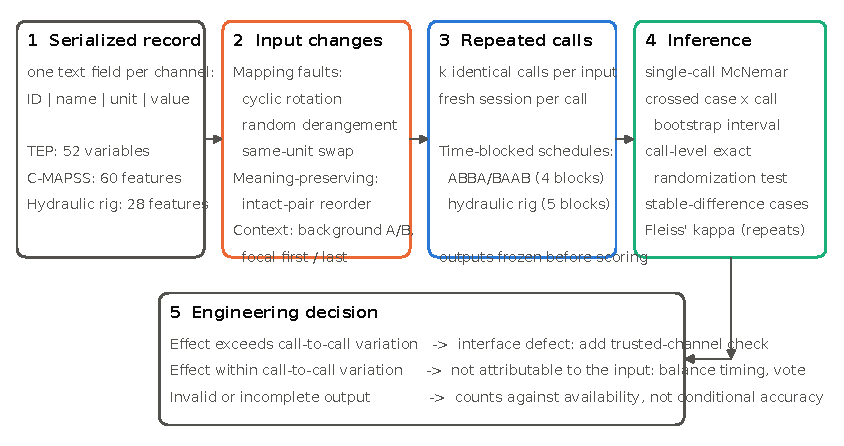
\includegraphics[width=\linewidth]{figures/v2/framework.pdf}
\caption{Repeated-call evaluation framework. Input changes are compared with identical-input repeats, while screening and voting are evaluated through released errors, coverage and call cost. The workflow evaluates possible checks rather than certifying deployment safety.}
\label{fig:framework}
\end{figure}

\subsection{Input changes}
Table~\ref{tab:interventions} lists the input changes. A \emph{mapping fault} replaces the descriptor $d_j$ of each affected position with the descriptor of another channel while keeping the numeric string and its position unchanged, so the channel identity, name and unit move together. We use a one-position cyclic rotation of all descriptors, three fixed random derangements, and a swap of two channels that share a unit (reactor level and separator level, both in percent); the last is the hardest to detect by unit checks. An \emph{intact-pair reorder} permutes whole descriptor--value pairs and keeps every physical association correct; it controls for a change in presentation without a change in meaning. A \emph{context change} keeps the focal records byte-identical and varies either the unlabelled background records in the same request (panel A or B) or the focal block's position before or after the background, with request size held fixed. Within each study, permutations and panels were fixed before its new calls; later studies were informed by earlier results and are reported individually rather than selected by outcome.

\begin{table}[htbp]\centering\small
\caption{Input changes, the quantities they hold fixed and the question each answers.}
\label{tab:interventions}
\begin{tabularx}{\linewidth}{@{}>{\raggedright\arraybackslash}p{0.2\linewidth}>{\raggedright\arraybackslash}p{0.29\linewidth}>{\raggedright\arraybackslash}X@{}}\toprule
Change & Held fixed & Question \\\midrule
Mapping fault & Numeric strings and positions & Does the service respond to a wrong physical association? \\
Intact-pair reorder & Every descriptor--value pair & Is the decision sensitive to a meaning-preserving presentation change? \\
Background panel & Focal records, position, request size & Do co-presented unlabelled records change the focal labels? \\
Focal position & Focal records, background, request size & Does the position of the focal block change its labels? \\
Identical repeat & Entire request payload & How large is call-to-call variation? \\
\bottomrule\end{tabularx}\end{table}

\subsection{Repeated-call design}
Every condition is submitted $k$ times as separate calls in fresh sessions. On the source-disjoint TEP panel $k=3$ and all 84 calls follow one randomized schedule; because the order was random rather than balanced, a condition can by chance fall into one period of the session. Later studies therefore use time blocks that each contain every condition: an ABBA/BAAB replication of the focal-position contrast (four blocks), a five-block hydraulic study with byte-identical duplicates, two paired-position studies on new hydraulic blocks and on a bearing rig (two rounds of three focal-first/focal-last pairs), an original prospective known-answer study (three blocks), and a new-panel follow-up (three blocks). Each experimental stage preserves its inputs and outputs. The prospective screening trial froze its protocol and scoring code before its first call and scored outputs after freezing them. Earlier stages had result-informed follow-ups; the hydraulic completion included an interim R3 analysis while R4--R5 were running, without changing the fixed schedule (Supplementary Appendix~G). These records are not a third-party preregistration.

\subsection{Statistical inference}\label{sec:stats}
For a contrast between a reference condition $L$ and a changed condition $R$ on $n$ shared cases, let $c^{L}_{is}\in\{0,1\}$ indicate whether call $s$ labels case $i$ correctly, and $\hat y^{L}_{is}$ the label itself. We report complementary analyses with different sampling units and assumptions; their significance levels are not interchangeable.

\paragraph{Single-call McNemar test.} For the prespecified primary call pair (repeat~1), the exact McNemar test compares the discordant counts $b=\#\{c^L_{i1}=1,c^R_{i1}=0\}$ and $c=\#\{c^L_{i1}=0,c^R_{i1}=1\}$ with a Binomial$(b+c,\tfrac12)$ distribution \citep{mcnemar1947note,dietterich1998approximate}. $p$-values are Holm-adjusted within each family of contrasts \citep{holm1979simple}. This is the test an evaluation with one call per condition would use; it treats different test-case pairs as independent while retaining the paired comparison within each case.

\paragraph{Case and call uncertainty.} The pooled accuracy difference
\begin{equation}
\Delta=\frac{1}{nk_L}\sum_{i,s}c^L_{is}-\frac{1}{nk_R}\sum_{i,s}c^R_{is}
\end{equation}
uses all repeats. For unblocked studies we use 10{,}000 pigeonhole bootstrap replicates \citep{owen2007pigeonhole}, resampling shared cases and, independently, calls within each condition. For matched-block studies the revised analysis resamples shared cases and complete execution blocks, retaining all condition calls and their multiplicities within a selected block. Supplementary Appendix~F also preserves the former independent-column bootstrap as a sensitivity analysis. Neither approach captures changes in unobserved services or devices; with few blocks or calls, percentile intervals have limited resolution.

\paragraph{Call-level tests.} A whole-call comparison retains dependence among labels returned together. For the ABBA/BAAB replication, the original scheduler assigned exactly two ABBA and two BAAB sequences to four temporal blocks. The design-based test enumerates its six allowed assignments, under a sharp no-effect null and no carryover between requests. It does not enumerate arbitrary two-versus-two labels within each block. For other comparisons, we report the specified whole-call or within-block exchangeability test, conditional on the sampled schedule; validity requires the corresponding exchangeability assumption. With three unblocked calls per condition there are $\binom{6}{3}=20$ assignments and the minimum two-sided $p$ is 0.10. Consequently, disagreement with a single-call $p<0.05$ is not an estimated false-positive rate. The single-call audit reports both raw and Holm-adjusted results and explicitly labels its exploratory composite support convention.

\paragraph{Label disagreement and repeatability.} For case $i$, let $W_i$ be the mean disagreement $\mathbf 1(\hat y_{is}\neq\hat y_{it})$ over all within-condition call pairs and $B_i$ the mean over all between-condition pairs. The excess disagreement
\begin{equation}
E=\frac1n\sum_i (B_i-W_i)
\end{equation}
is zero in expectation when the calls are exchangeable; a positive value means that labels differ more between conditions than between identical requests. We report a case-bootstrap interval for $E$ and its one-sided call-level randomization $p$-value. A case is a \emph{stable difference} when all calls in each condition agree but the two conditions give different labels. Repeatability of identical calls is summarized by Fleiss' $\kappa$ \citep{fleiss1971measuring}. Accuracy intervals for single calls use the Wilson method \citep{wilson1927probable}.

\subsection{Error structure}\label{sec:structure}
For $k$ byte-identical calls on $n$ focal cases, a case is \emph{always correct} if every call labels it correctly, \emph{always wrong} if no call does, and of \emph{mixed correctness} otherwise. Always-wrong cases are further separated into those with one persistent wrong label and those switching between wrong labels. This distinction matters: the first group passes agreement checks, whereas the second can be rejected by unanimity or pairwise agreement. Voting cannot recover a true label that was absent from every sampled response, but this does not imply that an abstention policy cannot reject that case.

The share of observed error instances contributed by always-wrong cases is
\begin{equation}
s=\frac{k\,n_{\mathrm{AW}}}{\sum_{i,s}(1-c_{is})}.
\end{equation}
For plurality aggregation, $1-s$ bounds the normalized gain in usable correct yield, $G=(Y_{\mathrm{plurality}}-A_{\mathrm{single}})/(1-A_{\mathrm{single}})$, because always-wrong cases cannot contribute correct output. Ties count as non-correct yield here, not as released diagnostic errors. Thus a relation between this share and same-sample voting performance is partly an accounting constraint, not independent validation of a policy-selection rule. A \emph{whole-call failure} denotes a response with errors on many records together; it is distinct from the directly observable \emph{label concentration} of that response. Low concentration does not establish correctness, and high concentration may be appropriate in an unbalanced real batch.

\subsection{Known-answer screening and decision policies}\label{sec:canary}
Each request contains focal records and reference (\emph{canary}) records whose labels are known to the operator but withheld from the model. The screen accepts a call if reference accuracy is at least $\tau=0.8$; with nine canaries this requires eight correct. The prospective trial fixed this threshold before calls. Applications to earlier studies and the new label-concentration control are post hoc analyses. A shared response failure can affect both groups, allowing reference errors to flag unreliable focal labels; the association is an empirical question, not guaranteed by sharing a request.

Policies operate on windows of repeated calls for one batch. \emph{Single} uses the earliest dispatched call. \emph{Canary} uses the first passing call in verified dispatch order, or withholds all focal decisions if the budget is exhausted. The prospective trial allows three attempts per arm-by-block window. \emph{Vote} selects the most frequent label; historical analyses abstain on any tie for highest count. The prospective trial's original tie rule selects the first-call label among tied leaders; tie-abstention is separately reported as a post hoc sensitivity. Historical windows contain 3--10 calls, rather than uniformly three. A failed or missing attempt consumes its slot and does not trigger a replacement.

\emph{Collapse-only} follows the same three-attempt first-passing policy, rejecting a response if at least 90\% of all 27 output labels are identical. It reads no reference answers. This control and its 85\%, 95\% and 100\% threshold sensitivities were specified after the prospective outcomes were available, before computing the control comparison; none is selected to maximize performance. Both screens use the identical requests, which isolates the acceptance information without changing batch size. Their input cost includes the reference records, even though Collapse-only does not read their labels.

For paired-position studies, \emph{Same} and \emph{View} keep a first-call label only if a second identical call or a changed-position call agrees. These use a smaller focal-first subset and are not directly ranked against full-window policies. We report coverage and accepted-label error \citep{geifman2017selective}, together with usable correct yield and calls per \emph{window}, not per individual diagnosis. Chronological corrections and request-level selections are retained in the supplementary audit.

\subsection{Trusted-channel gateway}
A trusted-channel gateway checks every descriptor against a registry keyed by acquisition channel IDs, rejects unknown, duplicate or inconsistent descriptors and writes accepted records in a canonical order. The acquisition IDs are not passed to the model, so they cannot act as a second, uncorrupted identity. The gateway is tested on clean inputs, intact reorderings, the two visible descriptor faults and a hidden value swap that exchanges the values of two same-unit channels while leaving the descriptors intact; such a swap is internally consistent and therefore invisible to any metadata check.

\section{Experimental setup}\label{sec:setup}
\subsection{Datasets and panels}
Table~\ref{tab:data} summarizes the evaluation panels.

\emph{Tennessee Eastman Process.} We use the expanded TEP simulation data of \citet{rieth2017additional} for the benchmark process of \citet{downs1993plant}, with 52 measured and manipulated variables and seven classes: normal operation and faults 1, 2, 4, 6, 7 and 13. Training, development and all earlier evaluation runs were excluded globally, and 112 of the remaining 135 run IDs were drawn without inspecting predictions. Seventy runs, ten per class, form the main panel; we keep simulation runs disjoint across training and evaluation, and each main-panel run contributes one seeded late snapshot (sample index 200--500). Two disjoint background panels, A and B, contain 21 runs each (three per class). A fixed focal subset of 21 main-panel runs, three per class, is used for the context contrasts. The same 70 runs at sample 40, about one hour after fault injection, form the early-stage transfer panel.

\emph{C-MAPSS.} For FD001 and FD002 \citep{saxena2008damage,saxena2008dataset}, each engine is summarized over its last 30 available cycles by the mean, population standard deviation, least-squares slope and last value of 15 training-selected channels (60 features). Three retrospective health classes are defined from true remaining useful life (RUL): Healthy (RUL $>80$), Degrading ($30<\text{RUL}\le80$) and Critical (RUL $\le30$). FD001 uses 60 held-out engines and FD002 60 test engines, 20 per class, from the six-operating-condition subset. The FD001 representation is applied unchanged to FD002; operating settings are not included.

\emph{Hydraulic test rig.} The UCI condition-monitoring dataset \citep{helwig2015hydraulicdata,helwig2015condition} contains 2{,}205 measured 60-s cycles from one physical rig. The task is internal pump leakage (no, weak, severe). Because cooler states occupy three contiguous time segments, every panel is balanced over all nine pump $\times$ cooler strata, and the earlier panels take one middle stable cycle from each selected block of constant component conditions; the follow-up exception is described below. Each cycle is described by the mean and population standard deviation of 14 physical sensors (28 features); the virtual efficiency channels are excluded. The focal panels of the first three hydraulic studies use disjoint blocks; reference records are reused where stated. The \emph{five-block study} uses three 18-cycle panels (focal, A and B) and a record-wise \texttt{descriptor=value} serialization. The \emph{new-block study} draws 27 focal and 27 background cycles from 54 previously unused blocks, forms three panels of nine plus nine, and uses a compact serialization with one shared feature dictionary and value arrays. The \emph{prospective known-answer study} draws 18 focal cycles from unused blocks and nine canaries, one per stratum, from the five-block focal panel. The subsequent \emph{stability follow-up} uses the remaining 18 eligible unused blocks: nine focal blocks contribute two separated stable cycles each and nine other blocks contribute one reference cycle each. Its 18 focal records therefore represent nine source blocks, not 18 independent sources.

\emph{Paderborn bearing rig.} The Paderborn data \citep{lessmeier2016benchmark} contain motor-current and vibration recordings of healthy bearings and of bearings with inner- or outer-race damage produced in accelerated-life tests. Nine focal bearings, three per class, each contribute one recording under each of four operating regimes (36 records), and six other bearings contribute 12 background recordings. Seven channels (radial force, two phase currents, speed, temperature, torque and vibration) give 28 features: means and standard deviations, the RMS, crest factor and kurtosis of the three high-rate signals, and five relative vibration-band powers. These fixed summaries omit bearing-geometry-specific envelope features, so the study tests the interface rather than an optimized bearing-diagnosis pipeline.

\begin{table}[htbp]\centering\small
\caption{Evaluation panels. Calls count separate requests; repeated labels of the same case are not independent observations.}
\label{tab:data}
\begin{tabularx}{\linewidth}{@{}l>{\raggedright\arraybackslash}p{0.17\linewidth}>{\raggedright\arraybackslash}p{0.2\linewidth}r>{\raggedright\arraybackslash}X@{}}\toprule
Panel & Classes & Cases & Features & Calls \\\midrule
TEP late (main) & Normal + 6 faults & 70 & 52 & 3 per condition and service (7 mapping conditions) \\
TEP focal context & Normal + 6 faults & 21 (+21 background) & 52 & 3 per context; ABBA/BAAB: 16 \\
TEP early & Normal + 6 faults & 70 & 52 & 3 per service \\
C-MAPSS FD002 & 3 health classes & 60 & 60 & 3 per service \\
Hydraulic, five-block & 3 leakage levels & 18 (+36 background) & 28 & 5 blocks $\times$ 9 conditions + 18 single-record \\
Hydraulic, new blocks & 3 leakage levels & 27 (+27 background) & 28 & 36 (2 rounds $\times$ 3 panels $\times$ 3 F/R pairs) \\
Hydraulic, prospective & 3 leakage levels & 18 (+9 canaries) & 28 & 27 (3 blocks $\times$ 3 arms $\times$ 3) \\
Hydraulic, stability & 3 leakage levels & 18 from 9 blocks (+9 new canaries) & 28 & 18 (3 blocks $\times$ 2 arms $\times$ 3) \\
Paderborn bearing & healthy, inner, outer & 36 (+12 background) & 28 & 12 (2 rounds $\times$ 3 F/R pairs) \\
\bottomrule\end{tabularx}\end{table}

\subsection{LLM services and execution}
Two services were evaluated in full: \texttt{gpt-5.6-sol} (Sol) and \texttt{gpt-6-astra} (Astra), both called through the Codex command-line interface (version 0.155.0-alpha.9.2 in the original studies) with medium reasoning effort in the original experiments. Each call ran in a fresh, empty session with tools, plugins, web access and project context disabled. Requests contained anonymous eight-character IDs, the permitted labels and a short description of each fault mechanism, but no per-case labels, labelled examples or class quotas. Each scheduled job was invoked once with its study-specific timeout (300 s for ABBA/BAAB, 170 s for the paired hydraulic/bearing policies and 900 s for the hydraulic and canary trials); failed or invalid calls were retained. The separate hydraulic completion reran the incomplete R3 block in full; its three earlier valid R3 responses remain archived and are excluded from the completion analysis, rather than silently replaced. Temperature is not exposed by this interface, and the requested model aliases do not guarantee a fixed server-side snapshot, so all results refer to the recorded call windows.

A preliminary 130-source panel (60 FD001 engines and 70 TEP runs) had evaluated five services with clean and rotated descriptors (Supplementary Sections~3 and~5). There, the rotation reduced primary TEP accuracy by 77.1 points for Sol, 28.6 for GPT-5.5 and 22.9 for Qwen3.8-Max, left Astra's labels unchanged, and caused two of three DeepSeek-V4-Pro corrupted-TEP responses to exhaust the output budget. These results motivated the source-disjoint study but are not pooled with it.

The source-disjoint TEP study comprised 84 calls (two services, 14 conditions, three repeats) and 4{,}854 classification slots, and the ABBA/BAAB replication added 16 Sol calls. The five-block hydraulic study scheduled 63 Sol calls. Its first run stopped in block R3 after two network time-outs; a versioned completion executed blocks R3--R5 in full with byte-identical prompts, so every analysed block contains contemporaneous controls (Supplementary Appendix~G). The new-block hydraulic and bearing studies used Sol in two sequential rounds; in each round every panel received three pairs of calls, one with the focal block first (F) and one with it last (R), launched in randomized slots on a fixed 180-s grid (36 and 12 calls; Supplementary Appendix~I). All later studies used Sol only, because it had shown the larger call-to-call variation; this result-informed choice supports no ranking of services.

\paragraph{Prospective known-answer study.}\label{sec:prospective} This study was designed after the retrospective analyses of Section~\ref{sec:canary_results} and frozen, together with its scoring code, before any call. Each request contains the 18 new focal cycles and nine canaries interleaved in one fixed random order and uses the five-block serialization. Three arms differ only in the serialization: canonical field order (C); an upstream hidden swap of the PS1 and PS2 values in every record (H), which the gateway accepts; and intact-pair reversal (R). Three contiguous blocks each contain three byte-identical calls per arm in random order (27 calls, 729 slots). The prespecified endpoints are the correlation between canary and focal accuracy over calls (one-sided permutation test), the focal accuracy of accepted against rejected calls, screen-and-retry within each arm-by-block window against its first call and a three-call vote, and the effect of the hidden swap on focal accuracy and on canary rejection.

\paragraph{New-panel stability follow-up.} After the original trial and its post hoc concentration control, both rules, all thresholds, source exclusions, the scoring code and the 18-call schedule were fixed on 30 September 2026 before the first new call. Canonical (C) and intact-reversal (R) arms each receive three calls per chronological block over three blocks, giving six policy windows. The hidden-swap arm is omitted; like-arm comparisons therefore restrict the earlier trial to C/R. All 27 records and 18 source blocks are new relative to previous hydraulic selections. Two spaced focal cycles are selected per focal block without examining predictions; the new references occupy different blocks. The fixed focal nuisance setting is valve 100/accumulator 100 and the reference setting valve 90/accumulator 100. This changes source panel, reference panel and service period together, and the CLI changes from 0.155.0-alpha.9.2 to 0.159.0; no unchanged model snapshot is claimed. Each job is invoked once, with no replacement. The full collection is completed before scoring, permitting offline replay under a shared maximum three-call budget for both screens and voting (Supplementary Appendix~M).

\subsection{Supervised baselines}
Six supervised classifiers were trained with scikit-learn \citep{pedregosa2011scikit}: a random forest (RF) \citep{breiman2001random}, an RBF support vector machine, histogram gradient boosting (HGB), a multilayer perceptron, $k$-nearest neighbours and multinomial logistic regression. They receive the same rounded features and test cases as the LLM but also use labelled training data. Hyperparameters were chosen by five-fold GroupKFold cross-validation on the training data only, grouped by training run or engine and scored by macro-F1. In the \emph{like-for-like} setting, the classifiers are trained on late snapshots of the 100 TEP training runs and on the 100 FD001 training engines, using the source domains available when the LLM prompts were designed, but with labelled fitting data not supplied in the LLM requests, and are then applied unchanged to every panel. Two further settings give the classifiers target-domain information that the LLM never receives: a \emph{phase-aware} TEP model trained on both late and sample-40 snapshots of the training runs, and FD002 models trained on 260 FD002 training engines after operating-regime normalization (six regimes found by $k$-means on the operating settings, following earlier C-MAPSS preprocessing strategies reviewed by \citet{ramasso2014benchmarking}). No test run or engine occurs in any training set. Because the best method differs between panels, we report the range over all six methods rather than a single reference chosen on test scores; per-method results and hyperparameters are in Supplementary Appendix~H.

For the bearing task, an RBF SVM and a random forest were fitted, after the LLM results were known, on 120 recordings from the six background bearings, tuned by bearing-disjoint validation and tested on the 36 focal recordings from the nine held-out bearings with the same 28 features; a second fit also held out each operating regime in turn. No test bearing entered fitting or tuning (Supplementary Appendix~J).

\subsection{Metrics}
We report accuracy, macro-F1, the number of changed labels between paired calls, the statistics of Section~\ref{sec:stats}, request validity, token usage and latency. Accuracy is conditional on a valid response; availability is reported separately as valid classification slots over scheduled slots.

\section{Results}\label{sec:results}
\subsection{Prospective screening: benefit, rejection and retry cost}\label{sec:prospective_results}
All 27 calls of the locally frozen prospective trial were valid, generating 729 classifications and using 603{,}721 input-plus-output tokens. The 18 focal cycles and nine reference cycles were reused across calls; the policy comparison comprises nine arm-by-block windows, or 162 focal decision slots, rather than 162 independent cycles. Eleven calls passed the eight-of-nine reference threshold. Their focal accuracy was 190/198 (96.0\%), versus 120/288 (41.7\%) in the 16 rejected calls. Canary and focal accuracy were associated (Spearman $\rho=0.971$); the prespecified 10{,}000-draw unrestricted permutation procedure gave $p=1/10001$. This is a Monte Carlo reference under exchangeability, not exact enumeration. A post hoc within-arm-by-block permutation sensitivity gave the same minimum Monte Carlo value, without establishing independence of the repeated cycles (Supplementary Appendix~K).

Under the fixed three-attempt budget, Canary selected seven calls across nine windows. It released 123 correct and three incorrect labels, withheld 36 decisions and used 17 calls. Single released 105 correct and 57 incorrect labels using nine calls. Thus accepted-label error decreased from 35.2\% to 2.4\%, coverage decreased from 100\% to 77.8\%, and usable correct yield increased from 64.8\% to 75.9\%. The additional eight calls bought 18 additional correct outputs while reducing released errors by 54. The three errors that passed the screen show that reference success does not certify every focal diagnosis. Per-call and per-window records in Supplementary Appendix~K expose which windows were accepted and which exhausted their budgets.

The prespecified three-call Vote with first-call tie resolution produced 102/162 correct labels (63.0\%). The separately reported tie-abstention sensitivity produced 97 correct, 59 incorrect and six withheld labels (59.9\% usable correct yield; 37.8\% accepted error). Repeated voting therefore did not improve the first-call result in this trial. All 27 requests were collected to compare policies; the 17-call screening cost is a replay of the fixed policy on that sequence, not a claim that collection stopped after 17 requests.

The hidden PS1/PS2 swap arm scored 58.6\% versus 53.1\% for canonical serialization (within-block comparison $p=0.72$); reference rejection was 67\% versus 78\%. This endpoint did not establish harmful-fault detection or equivalence. The observed screening benefit concerns poorly performing calls, without proving that the screen verifies sensor mappings.

\paragraph{A label-free collapse control.}

A post hoc control tests whether known canary labels add value beyond detecting near-monolabel outputs. Using the same frozen calls, payloads and three-call windows, it rejects a request when at least 90\% of its 27 labels agree (25 or more), without reading reference labels or record roles. The rule and 85\%, 95\% and 100\% sensitivities were fixed before computing this control, after the original outcomes had been inspected; this is not an independent prospective validation.

\begin{table}[htbp]\centering\small

\caption{Post hoc control on nine prospective-study windows. Calls/window count requests an offline policy would require; all 27 source calls were collected.}\label{tab:canary_control_main}

\begin{tabular}{lrrrrr}\toprule

Policy & Correct & Error & Withheld & Coverage (\%) & Calls/window \\ \midrule

Single & 105 & 57 & 0 & 100.0 & 1.00 \\

Known answer & 123 & 3 & 36 & 77.8 & 1.89 \\

Collapse only (90\%) & 123 & 3 & 36 & 77.8 & 1.89 \\

Three-call vote & 102 & 60 & 0 & 100.0 & 3.00 \\

\bottomrule\end{tabular}\end{table}

The 90\% collapse control and known-answer policy select the same calls in every window and therefore have identical retained labels and required-call resources. Incremental window-level benefit from knowing the canary labels is not established. At the call level, collapse screening additionally passes two noncollapsed calls containing 12 focal errors among 36 outputs; neither is selected by the first-passing window rule. The 85\% rule gives the same window outcomes, whereas 95\% and 100\% reproduce Single. Supplementary Appendix~L reports acceptance cross-tabs, tie sensitivity and resources. Because every request retains the canary records, this comparison isolates label use at the decision stage; it does not test removing those records from prompts.


\paragraph{Prospectively fixed later-period follow-up.}
After specifying the collapse control, we froze the same screening thresholds and scorer for a fresh 18-request follow-up on 30 September. The unchanged hydraulic rig supplies 18 new focal cycles from nine previously unused source blocks (two spaced cycles per block), plus nine new canaries from nine other unused blocks. Canonical (C) and intact-pair reversal (R) each receive three byte-identical calls in each of three chronological blocks. The source panel, canary panel, service period and client version change jointly; this is not a separate causal test of any one change or a new-device replication.

\begin{table}[htbp]\centering\small
\caption{Later-period follow-up on six C/R windows. All four policies cover 108 window decisions on the same 18 focal cycles; calls are offline required requests, not actual adaptive savings.}
\label{tab:canary_stability_main}
\begin{tabular}{@{}lrrrr@{}}\toprule
Policy & Correct & Error & Withheld & Calls/window \\\midrule
Single & 88 & 20 & 0 & 1.00 \\
Known answer & 100 & 8 & 0 & 1.50 \\
Collapse only (90\%) & 88 & 20 & 0 & 1.00 \\
Three-call vote & 84 & 24 & 0 & 3.00 \\
\bottomrule\end{tabular}\end{table}

Known-answer screening retains 100 correct and eight incorrect labels among 108 window decisions (92.6\% correct yield and 7.4\% accepted-case error), compared with 88 correct and 20 incorrect for Single and the 90\% collapse control. All three policies cover every window decision. This descriptive gain requires nine calls rather than six (1.50 versus 1.00 per window), corresponding to 206,117 rather than 135,535 observed input-plus-output tokens in the offline replay. The full study actually collected all 18 calls and used 408,408 tokens.

Every new call passes the collapse rule: its modal class occupies only 9--15 of 27 labels. Known-answer screening rejects ten of those calls. Its window-level gain is concentrated in C/block~2 (+10 correct) and R/block~3 (+2); the other four windows are unchanged. Thus reference labels provide discrimination beyond this fixed collapse check in the new sample, but these six dependent windows do not establish a population benefit. All eight retained errors repeat two weak-leakage cycles from one source block, classified as no leakage in four selected calls. The guard therefore does not assure correctness for every source even when its reference check passes. Supplementary Appendix~M gives all 18 calls, six windows, retained errors, and comparisons restricted to the earlier study's matching C/R arms.


\subsection{Clean accuracy and transfer}
Table~\ref{tab:transfer} compares the two services with the supervised references on clean inputs. On late-stage TEP snapshots both services were almost perfectly accurate, but so were RF and HGB, so this panel shows no advantage for the LLMs. On FD001, tuned HGB reached 85.0\% against 71.7\% for Astra's primary call (McNemar $p=0.096$).

\begin{table}[htbp]\centering\small
\caption{Clean-input accuracy (\%) of the LLM services (three calls) and of six supervised references. Same-feature references additionally use labelled training data; the last column gives references that also receive target-domain information (TEP: phase-aware training with sample-40 snapshots; FD002: in-domain training with regime normalization). Ranges are over the six methods. McN: exact McNemar $p$, Astra call~1 versus HGB in the same setting.}
\label{tab:transfer}
\setlength{\tabcolsep}{4pt}
\begin{tabular}{@{}lccccc@{}}\toprule
Panel & Sol (calls 1/2/3) & Astra (calls 1/2/3) & Like-for-like & McN & With target info (McN) \\\midrule
TEP late & 100.0/97.1/100.0 & 100.0/100.0/100.0 & 77.1--100.0 & 1.00 & 78.6--100.0 (1.00) \\
TEP early & 87.1/85.7/88.6 & 88.6/87.1/88.6 & 22.9--54.3 & $1.2\times10^{-7}$ & 74.3--88.6 (1.00) \\
FD001 & 71.7/68.3/70.0 & 71.7/73.3/75.0 & 68.3--85.0 & 0.096 & -- \\
FD002 & 60.0/26.7/56.7 & 71.7/76.7/78.3 & 33.3--45.0 & 0.007 & 81.7--86.7 (0.035) \\
\bottomrule\end{tabular}\end{table}

The two transfer panels show where the LLMs helped and why. On early TEP snapshots, about one hour after fault onset, every like-for-like reference fell to 22.9--54.3\%, while both services stayed at 86--89\%; Astra was correct on 24 cases where HGB was wrong and never the reverse ($p=1.2\times10^{-7}$). Trained with early snapshots as well, the references reached 74.3--88.6\%, and HGB no longer differed from Astra ($p=1.00$). On FD002, the like-for-like references reached at most 45.0\%, below Astra's 71.7\% ($p=0.007$). With in-domain training and regime normalization they reached 81.7--86.7\% and HGB outperformed Astra ($p=0.035$); regime normalization alone, estimated from unlabelled FD002 data and applied to the FD001-trained references, gave 71.7--86.7\%. The observed advantage depended on the training-resource comparison and disappeared once the classifiers were given target-domain information; it does not isolate the cause of the services' transfer behaviour. The services differed sharply in repeatability under operating-condition shift. On FD002, Sol's three calls returned 60.0, 26.7 and 56.7\% accuracy with Fleiss' $\kappa=0.08$; only 10 of 60 engines received the same label in all three calls. Astra's calls were far more consistent ($\kappa=0.90$; 71.7--78.3\%). For Sol, a single FD002 call is thus a poor estimate of what the next call will return.

No method solved the bearing task. Sol's twelve calls classified 4--16 of the 36 focal recordings correctly, 13.9\% of the focal labels in focal-first calls and 31.0\% in focal-last calls, against 33.3\% by chance. The supervised references did no better on the held-out bearings: 10/36 for the SVM and 4/36 for the random forest, below the 12/36 of a constant prediction, and 13/36 and 9/36 when the operating regime was also held out, although their bearing-disjoint validation accuracies during tuning had been 85.4\% and 76.7\%. With six development bearings, these fixed summaries support cross-bearing diagnosis for neither kind of model. The bearing study therefore serves below as a test of how checks behave when the underlying task fails.

\subsection{Descriptor-mapping faults}
Table~\ref{tab:mapping} and Figure~\ref{fig:forest}(a) report the mapping contrasts on the 70-run panel; Figure~\ref{fig:repeats} shows every call. The cyclic rotation reduced Sol's accuracy from 99.0\% to 40.5\% over three calls each ($\Delta=58.6$ points, 95\% CI 37.1--77.1). The effect was large at every level of analysis: 47 of 70 labels changed in the primary call pair (McNemar $p=1.4\times10^{-14}$), the excess disagreement was $E=0.37$ (95\% CI 0.27--0.48), and the call-level randomization test reached its smallest attainable value, $p=0.10$. Twenty cases were stable differences, correct in all three clean calls and consistently wrong in all three rotated calls. The rotation also made Sol less repeatable: Fleiss' $\kappa$ fell from 0.98 on clean inputs to 0.49.

\begin{table}[htbp]\centering\small
\caption{Mapping contrasts on 70 source-disjoint TEP runs (three calls per condition). $\Delta$: pooled clean-minus-changed accuracy (percentage points) with 95\% crossed bootstrap CI. McN: exact McNemar $p$ for repeat~1, Holm-adjusted over six contrasts. Rand.: two-sided call-level randomization $p$ (20 reassignments; minimum 0.10). $E$: excess disagreement. SD: stable-difference cases. $\kappa$: Fleiss' kappa of the changed condition (clean: Sol 0.98, Astra 1.00).}
\label{tab:mapping}
\setlength{\tabcolsep}{4pt}
\begin{tabular}{@{}llrrrrrrr@{}}\toprule
Service & Change & Acc. (\%) & $\Delta$ [95\% CI] & McN $p$ & Rand. $p$ & $E$ & SD & $\kappa$ \\\midrule
Sol & Cyclic rotation & 40.5 & 58.6 [37.1, 77.1] & $<10^{-13}$ & 0.10 & 0.371 & 20 & 0.49 \\
Sol & Random 1 & 80.0 & 19.0 [$-2.9$, 56.7] & 1.00 & 1.00 & $-0.003$ & 0 & 0.53 \\
Sol & Random 2 & 88.6 & 10.5 [$-1.9$, 28.6] & 1.00 & 0.70 & 0.002 & 0 & 0.74 \\
Sol & Random 3 & 86.7 & 12.4 [$-1.9$, 34.3] & $1.5\times10^{-7}$ & 0.70 & 0.002 & 0 & 0.69 \\
Sol & Same-unit swap & 90.0 & 9.0 [$-1.9$, 25.7] & 1.00 & 0.70 & $-0.002$ & 0 & 0.77 \\
Sol & Intact-pair reorder & 99.0 & 0.0 [$-2.9$, 2.9] & 1.00 & 1.00 & $-0.003$ & 0 & 0.98 \\\midrule
Astra & All six changes & 100.0 & 0.0 [0.0, 0.0] & 1.00 & 1.00 & 0.000 & 0 & 1.00 \\
\bottomrule\end{tabular}\end{table}

The random derangements and the same-unit swap behaved differently. Each produced some low-accuracy calls (for example 40.0\% in the third call of derangement~1 and 62.9\% in the first call of derangement~3), but the other calls of the same input were near-perfect. For derangement~3 the primary-call McNemar test was highly significant (26 changed labels, Holm $p=1.5\times10^{-7}$), yet the pooled interval included zero, the randomization $p$ was 0.70 and no case was a stable difference. A single-call evaluation would have reported this as a strong mapping effect; the repeated calls show that the damage was confined to individual calls. What the faults did change consistently was repeatability ($\kappa$ 0.53--0.77 against 0.98 for clean inputs). The intact-pair reorder left both accuracy and repeatability unchanged, supporting a distinction between the tested incorrect mapping and the tested intact reorder, without covering all possible reorderings.

Astra returned identical, correct labels in all 21 calls on the mapping panel, including every mapping fault. On the preliminary panel it was likewise unaffected by rotation and by descriptor removal. This invariance is useful but should not be read as correct semantic use of the descriptors: a service that ignores the descriptors, relies on value patterns and field positions, or silently repairs a mapping would produce the same output. For the purpose of interface validation, the practical conclusion is that correct labels under a wrong mapping give no evidence that the mapping was checked.

\begin{figure}[htbp]
\centering
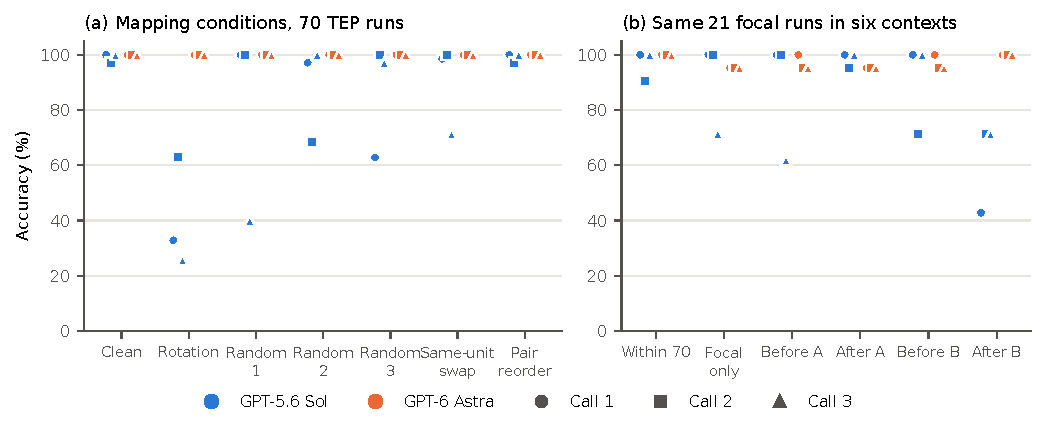
\includegraphics[width=\linewidth]{figures/v2/repeats.pdf}
\caption{All three calls of every mapping condition (a) and every context condition (b) on the source-disjoint TEP panel. Colour identifies the service and marker shape the call. Panel (b) scores only the same 21 focal runs in each request.}
\label{fig:repeats}
\end{figure}

\begin{figure}[htbp]
\centering
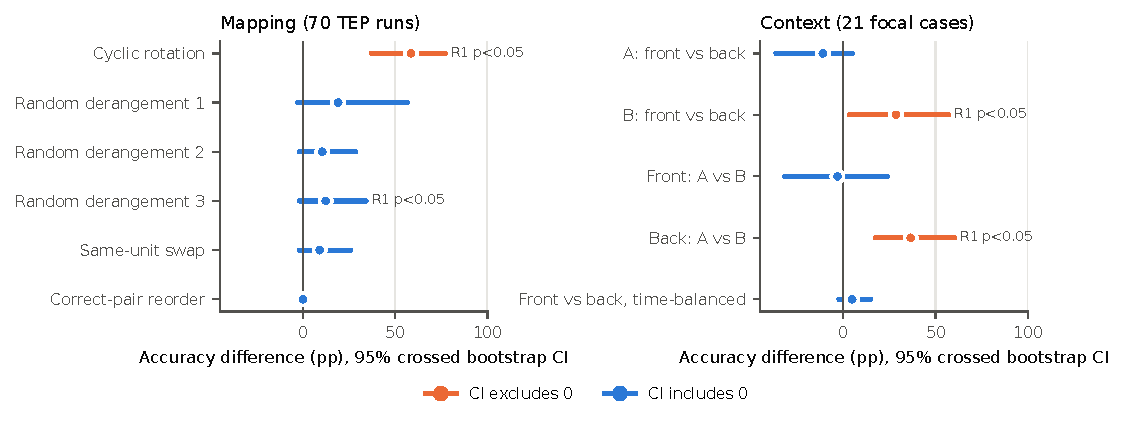
\includegraphics[width=\linewidth]{figures/v2/forest.pdf}
\caption{Pooled accuracy differences for GPT-5.6 Sol with 95\% bootstrap intervals: crossed case-by-call for the unblocked contrasts, and case-by-matched-block for ABBA/BAAB. ``R1 $p<0.05$'' marks contrasts whose primary-call McNemar test was significant after Holm adjustment. The last row of (b) is the time-balanced ABBA/BAAB replication.}
\label{fig:forest}
\end{figure}

\subsection{Context, position and call timing}
Table~\ref{tab:context} reports the four fixed-size context contrasts on the 21 focal runs and the time-balanced replication. Astra's focal labels changed by at most one case in any contrast. For Sol, the primary calls suggested a strong position effect: the focal runs were all correct when they preceded background B and only 9 of 21 were correct when they followed it (McNemar Holm $p=0.002$). The same focal records placed after background A were 21/21 correct, giving an equally significant background contrast.

\begin{table}[htbp]\centering\small
\caption{Context contrasts for Sol on the same 21 focal TEP runs (request size 42). Columns as in Table~\ref{tab:mapping}; McN is Holm-adjusted over the five contrasts in the original context family (including focal-only versus within-70). The ABBA/BAAB row pools eight calls per order in four blocks; the test uses the six sequence assignments allowed by the frozen design, and its interval resamples cases and matched blocks.}
\label{tab:context}
\setlength{\tabcolsep}{4pt}
\begin{tabular}{@{}lrrrrrr@{}}\toprule
Contrast (left vs right) & Acc. L / R (\%) & $\Delta$ [95\% CI] & McN $p$ & Rand. $p$ & $E$ & SD \\\midrule
A: focal first vs last & 87.3 / 98.4 & $-11.1$ [$-36.5$, 4.8] & 1.00 & 1.00 & $-0.011$ & 0 \\
B: focal first vs last & 90.5 / 61.9 & 28.6 [3.2, 57.1] & 0.002 & 0.30 & 0.063 & 0 \\
Focal first: A vs B & 87.3 / 90.5 & $-3.2$ [$-31.7$, 23.8] & 1.00 & 1.00 & $-0.063$ & 0 \\
Focal last: A vs B & 98.4 / 61.9 & 36.5 [17.5, 60.3] & 0.002 & 0.10 & 0.180 & 0 \\\midrule
ABBA/BAAB: first vs last (B) & 98.8 / 94.0 & 4.8 [$-3.6$, 16.1] & 0.50 & 0.67 & 0.003 & 0 \\
\bottomrule\end{tabular}\end{table}

The repeated calls do not support a position effect. Sol's two identical ``focal after B'' calls in repeats 2 and 3 disagreed on 12 of 21 labels while both scored 15/21, so identical-input variation was as large as the primary contrast. The B-position contrast had no stable-difference case, an excess disagreement whose interval included zero, and a randomization $p$ of 0.30. The only contrasts whose bootstrap intervals excluded zero were the two that involved the ``focal after B'' condition, and all three of its calls were started within the first 12 minutes of the session (Figure~\ref{fig:timing}a). In that early window, Sol's calls with intact mappings averaged 78.2\% accuracy (7 calls), against 96.5\% for the 11 calls started later. The trend was not significant on its own (Spearman $\rho=0.28$, $p=0.26$), so timing remains an alternative explanation: low-scoring calls were clustered in time, and the design does not isolate a service-period cause.

\begin{figure}[htbp]
\centering
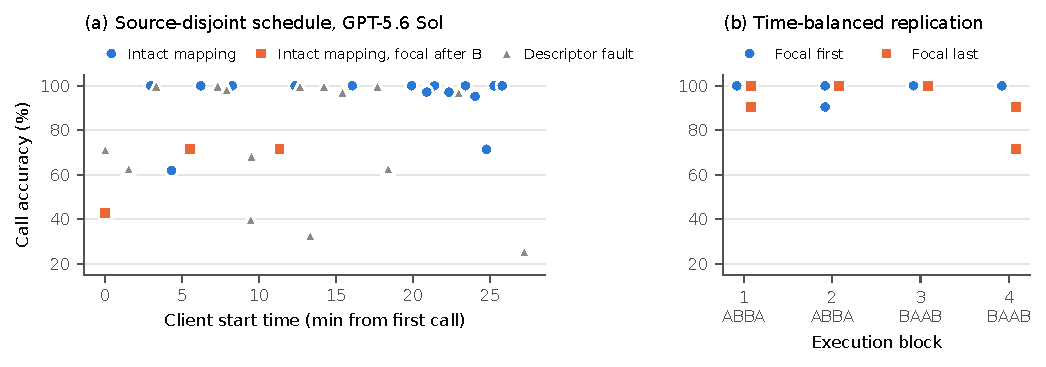
\includegraphics[width=\linewidth]{figures/v2/timing.pdf}
\caption{(a) Accuracy of every Sol call on the source-disjoint panel against its client start time. Intact-mapping calls (circles, squares) vary in accuracy; the three ``focal after B'' calls (squares) all started early. (b) Focal accuracy in the time-balanced ABBA/BAAB replication; each block contains two calls per order.}
\label{fig:timing}
\end{figure}

The ABBA/BAAB replication tested the B-position contrast directly. Its 16 calls were all valid. Focal-first calls averaged 98.8\% and focal-last calls 94.0\%, a difference of 4.8 points (95\% case-by-block interval $-3.6$ to 16.1). The design-based two-sided $p$ is $4/6=0.667$, using the six allocations of two ABBA and two BAAB sequences. The former 1{,}296-permutation calculation ($p=0.417$) assumes additional within-block exchangeability and is retained only as a sensitivity analysis. The largest discrepancy, 8 of 21 labels, occurred between identical focal-last calls in block~4 (Figure~\ref{fig:timing}b). The earlier 12/21 contrast was not reproduced; balancing and changes of service period are not separately identified. On new hydraulic blocks, focal-first and focal-last calls were correct on 128 and 139 of 162 focal labels ($-6.8$ points; sign-randomization $p=0.31$), and on the bearing rig on 30 and 67 of 216 ($-17.1$ points; $p=0.063$), while identical-input pairs differed by up to 7 of 9 and 22 of 36 labels, respectively.

\subsection{Measured hydraulic test rig}
All 63 scheduled calls of the five-block analysis set returned valid responses (1{,}278 classification slots). Table~\ref{tab:hydraulic} reports the contrasts and Figure~\ref{fig:hydraulic} every call. The results differ from TEP in one important respect: on measured data the presentation of the record mattered more than the correctness of the mapping.

With fields in canonical order, Sol classified the 18 focal cycles correctly in 40.0\% of cases, and its byte-identical duplicate in 44.4\%, close to the 33.3\% expected by chance for three balanced classes. These calls were consistently poor. Reversing the intact descriptor--value pairs raised accuracy to 84.4\%, a 42.2-point increase (95\% case-by-block interval 17.8--65.6). The within-block exchangeability test gave $p=0.004$. The cyclic descriptor rotation also raised accuracy, to 82.2\% ($p=0.008$). These results distinguish the two tested layouts from the canonical order; they do not establish that incorrect mappings are generally benign.

\begin{table}[htbp]\centering\small
\caption{Hydraulic rig: Sol on 18 focal cycles over five blocks. Byte-identical duplicates are pooled as reference where available. Intervals resample cases and complete matched blocks. Rand.: within-block whole-call exchangeability $p$ (243 assignments for two versus one calls, 32 for one versus one, and 7776 for two versus two). McN: primary R1 test, Holm-adjusted over nine contrasts. Negative $\Delta$ favours the changed condition.}
\label{tab:hydraulic}
\setlength{\tabcolsep}{4pt}
\begin{tabular}{@{}lrrrr@{}}\toprule
Contrast (reference vs changed) & Acc. ref / changed (\%) & $\Delta$ [95\% CI] & McN $p$ & Rand. $p$ \\\midrule
Canonical vs intact-pair reversal & 42.2 / 84.4 & $-42.2$ [$-65.6$, $-17.8$] & 0.057 & 0.004 \\
Canonical vs descriptor rotation & 42.2 / 82.2 & $-40.0$ [$-66.7$, $-17.8$] & 1.00 & 0.008 \\
Canonical vs identical duplicate & 40.0 / 44.4 & $-4.4$ [$-22.2$, 10.0] & 1.00 & 0.50 \\
Focal+A vs identical duplicate & 58.9 / 62.2 & $-3.3$ [$-31.1$, 24.4] & 1.00 & 1.00 \\
A: focal first vs last & 60.6 / 62.2 & $-1.7$ [$-30.6$, 26.7] & 0.23 & 1.00 \\
B: focal first vs last & 60.0 / 50.0 & 10.0 [$-33.3$, 50.0] & 0.094 & 0.88 \\
Focal first: A vs B & 60.6 / 60.0 & 0.6 [$-35.0$, 36.7] & 0.094 & 1.00 \\
Focal last: A vs B & 62.2 / 50.0 & 12.2 [$-24.4$, 45.6] & 0.23 & 0.50 \\
Focal only vs focal+A & 42.2 / 60.6 & $-18.3$ [$-36.7$, $-3.9$] & 1.00 & 0.028 \\
\bottomrule\end{tabular}\end{table}

\begin{figure}[htbp]
\centering
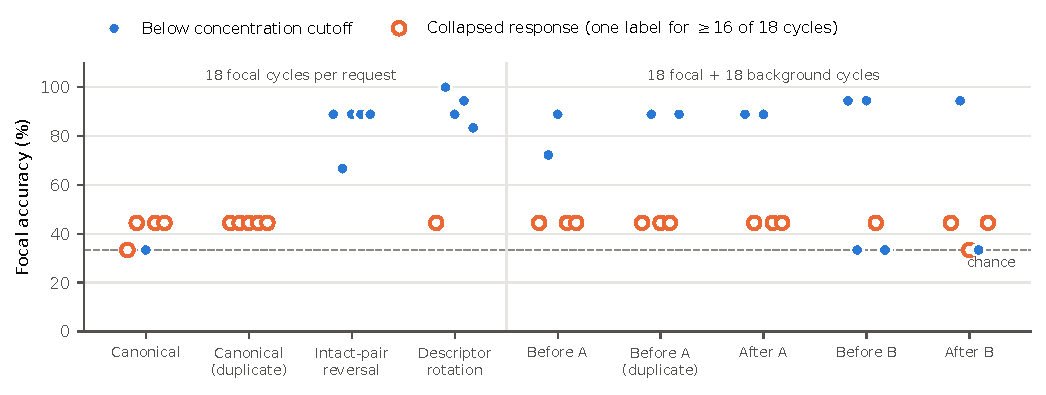
\includegraphics[width=\linewidth]{figures/v2/hydraulic.pdf}
\caption{Every Sol call on the measured hydraulic rig; the five points per condition are execution blocks R1--R5 from left to right. Open markers are collapsed responses that assign one label to at least 16 of the 18 focal cycles. Dashed line: chance level for three balanced classes.}
\label{fig:hydraulic}
\end{figure}

The per-call outputs explain the pattern. Sol's responses fell into two modes (Figure~\ref{fig:hydraulic}). In a \emph{collapsed} response it assigned one label, almost always ``no leakage'', to at least 16 of the 18 focal cycles; such calls averaged 43.5\% accuracy (23 calls). Otherwise the labels were spread over the three classes, and 18 of these 22 calls scored 12--18 correct. Collapse occurred in 9 of 10 canonical calls, in none of the 5 reversed calls and in 1 of 5 rotated calls. Historical Fisher comparisons are exploratory and do not model shared-panel or within-block dependence (Supplementary Appendix~G). These concentrated outputs accompanied poor focal accuracy in the sampled calls, with frequencies differing between the tested layouts. This descriptive pattern motivates the answer-free concentration control.

Context changes on the rig behaved as they had on TEP once calls were pooled. In block R1 all four fixed-size context contrasts had single-call McNemar $p<0.05$ before adjustment, yet none survived Holm adjustment and none had a randomization $p$ below 0.5. With 36 records per request, byte-identical calls alternated between about 8 and 16 correct focal cycles with some low-scoring responses nearly monolabel. Variation between these calls complicates interpretation of the single-call contrasts. Adding background A to the focal records raised accuracy from 42.2\% to 60.6\% ($p=0.028$), accompanied by a lower observed collapse frequency (9/10 against 13/25), but this comparison changes request size and composition together. The 18 single-record calls returned 7 correct labels (38.9\%).

The analysed hydraulic set used 1.24 million input-plus-output tokens. Median latency was 49~s per call (range 16--263~s), and even a single-record request consumed about 11{,}000 tokens because of the fixed instruction overhead of each fresh CLI session.

\subsection{Error structure across studies}\label{sec:structure_results}
Figure~\ref{fig:structure}(a) places the 28 identical-input groups with at least five errors, from all five studies, by the share of their errors that recurred in every call and by the normalized gain in usable correct yield from a plurality vote over their observed calls ($k=3,5,6,8$ or 10). The following groups are descriptive summaries of those same calls. In 13 groups errors varied between calls, and the normalized yield gain was 29--100\%: Sol's random derangements went from 80.0--88.6\% single-call accuracy to 98.6--100\%, and two of the three new hydraulic panels from 78--82\% to 100\%. In 10 groups at least 38\% of the errors recurred in every call, and the normalized yield gain was between $-3$ and 7\%: Sol's cyclic rotation, both services on the early TEP snapshots and on FD002, the canonical hydraulic layout, a new hydraulic panel with two consistently underestimated fault severities, and both bearing conditions. The remaining five groups had negative normalized yield gains ($-11$ to $-50$\%): four hydraulic context groups and the early TEP ``focal after B'' group. Low-performing calls need not be nearly monolabel; the hydraulic focal-before-B group included two calls with six correct focal labels and a modal count of only six of 18. Output concentration therefore captures only one failure pattern.

\begin{figure}[htbp]
\centering
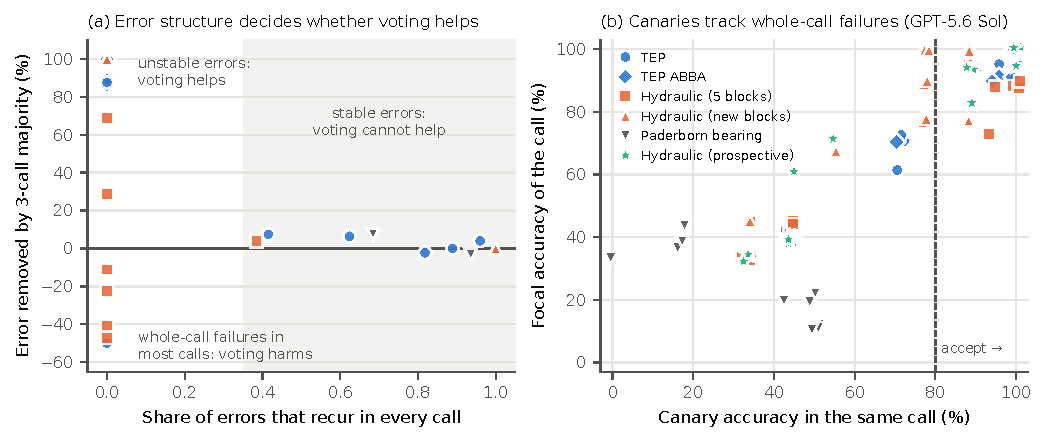
\includegraphics[width=\linewidth]{figures/v2/error_structure.pdf}
\caption{(a) Normalized usable-correct yield gain from a plurality vote across all available repeats against the share of error instances from always-wrong cases, for the 28 identical-input groups with at least five errors (both services; marker shapes as in b). (b) Canary accuracy against focal accuracy for every Sol call whose request contained labelled background or canary records; the dashed line is $\tau=0.8$, prespecified for the prospective trial and applied retrospectively to earlier studies. Stars mark the prospective study; small jitter separates overlapping calls.}
\label{fig:structure}
\end{figure}

The single-call audit concerns 19 overlapping Sol contrasts, not 19 independent experiments. With raw $p<0.05$, nine primary-call McNemar comparisons were nominally significant and six lacked the exploratory composite support criterion (call-level $p\le0.10$ and a nonzero bootstrap interval). With Holm correction, four were significant and two lacked that criterion. The tests have different units, assumptions and attainable $p$-values; lack of call-level support does not identify a single-call finding as false. Supplementary Appendix~F reports both conventions and the revised matched-block sensitivity. The useful observation is that an input-effect claim can change when repeated calls are considered, rather than that a measured fraction of tests is unreliable.

\subsection{Retrospective screening and policy comparisons}\label{sec:canary_results}
\paragraph{Retrospective analysis.} In the four studies in which the service could perform the task, the accuracy on the labelled background records tracked the accuracy on the focal records of the same call (Figure~\ref{fig:structure}b). The Spearman correlation over calls was 0.99 for the TEP context calls, 0.86 for the ABBA/BAAB calls, 0.81 for the five-block hydraulic calls and 0.75 for the new hydraulic blocks. Accepted calls were much more accurate than rejected ones: 99.3\% against 63.8\% on TEP and 88.9\% against 41.7\% in the five-block hydraulic study, where the screen separated collapsed from discriminating responses. On the bearing rig no call reached the threshold, because the service failed on the canaries as well as on the focal records; across its twelve calls the two accuracies were even negatively related ($\rho=-0.83$), so the screen could not rank calls there, only reject them all. These orderings held for every threshold between 0.6 and 1.0 (Supplementary Appendix~F); at 0.5, close to chance for three classes, seven bearing calls would have passed.

Table~\ref{tab:policies} compares the decision policies. Using actual dispatch timestamps in the five-block hydraulic study, screening lowered accepted error from 23/72 (31.9\%) for Single to 6/72 (8.3\%) and increased usable correct output from 49/72 (68.1\%) to 66/72 (91.7\%), using seven calls over four windows (1.75 per window). A former lexicographic repeat-order calculation selected later calls first and overstated this improvement; the revised chronology and selected request IDs are retained in the correction audit. On TEP it withheld the degraded ``focal after B'' window and accepted no error, but usable correct output decreased from 64/84 for Single to 63/84 for Canary. Where errors were unstable, as on the new hydraulic blocks, voting kept 98\% coverage with 10.4\% accepted error, whereas the screen reached 6.3\% at 58\% coverage; the Same and View checks accepted 10.8--11.4\% errors. On the bearing task, voting, Same and View still released wrong labels in 70--88\% of the decisions they accepted, while the screen withheld every decision. These retrospective comparisons motivated the prospective trial; they do not establish a universal improvement guarantee.

\begin{table}[htbp]\centering\small
\caption{Decision policies on windows of identical Sol calls whose requests contain canaries. Cov.: accepted over planned decisions. Err.: errors among accepted decisions. Yield: accepted correct over planned decisions. Calls: mean calls required per window by offline policy replay. Historical Vote abstains on any top-count tie; the prospective Vote uses the prespecified tie-first rule. Same and View are evaluated as in the original paired studies, on the first focal-first call of each panel and round (54 hydraulic and 72 bearing decisions).}
\label{tab:policies}
\setlength{\tabcolsep}{4pt}
\begin{tabular}{@{}llrrrrr@{}}\toprule
Study (decisions) & Policy & Cov. (\%) & Err. (\%) & Yield (\%) & Calls \\\midrule
TEP context (84) & Single & 100.0 & 23.8 & 76.2 & 1.00 \\
 & Vote & 100.0 & 14.3 & 85.7 & 3.00 \\
 & Canary & 75.0 & 0.0 & 75.0 & 1.75 \\\addlinespace
Hydraulic, five-block (72) & Single & 100.0 & 31.9 & 68.1 & 1.00 \\
 & Vote & 94.4 & 51.5 & 45.8 & 6.25 \\
 & Canary & 100.0 & 8.3 & 91.7 & 1.75 \\\addlinespace
Hydraulic, new blocks (108) & Single & 100.0 & 13.0 & 87.0 & 1.00 \\
 & Vote & 98.1 & 10.4 & 88.0 & 3.00 \\
 & Canary & 58.3 & 6.3 & 54.6 & 2.00 \\
\quad (54, first F call) & Same / View & 68.5 / 81.5 & 10.8 / 11.4 & 61.1 / 72.2 & 2.0 \\\addlinespace
Paderborn bearing (144) & Single & 100.0 & 75.0 & 25.0 & 1.00 \\
 & Vote & 97.9 & 72.3 & 27.1 & 3.00 \\
 & Canary & 0.0 & -- & 0.0 & 3.00 \\
\quad (72, first F call) & Same / View & 91.7 / 41.7 & 87.9 / 70.0 & 11.1 / 12.5 & 2.0 \\
\addlinespace
Hydraulic, prospective (162) & Single & 100.0 & 35.2 & 64.8 & 1.00 \\
 & Vote (tie-first) & 100.0 & 37.0 & 63.0 & 3.00 \\
 & Canary & 77.8 & 2.4 & 75.9 & 1.89 \\
\bottomrule\end{tabular}
\end{table}



\subsection{Trusted-channel gateway}
On all 54 measured hydraulic records of the five-block study, the gateway accepted every clean input and every intact-pair reversal and wrote them in identical canonical form. It rejected all 54 cyclic rotations and all 54 same-unit descriptor swaps without rejecting any clean input, and it accepted all 54 hidden value swaps, because a value moved together with a consistent descriptor looks like a real measurement at this layer. Canonical ordering also makes an intact-pair reorder byte-identical to the clean request; this removes one source of variation but does not make the output correct, since on the hydraulic rig the canonical order was the layout that collapsed most often. In the prospective study the gateway accepted the hidden-swap requests, as expected, but the experiment did not establish equivalence or reliable detection of a harmful swap (Section~\ref{sec:prospective_results}).

\section{Discussion}\label{sec:discussion}
\subsection{What the screen establishes}
The two prospective stages provide a bounded engineering result: a fixed reference screen with retries reduced released errors and increased correct outputs on the sampled hydraulic cycles. In the original trial it withheld two windows; in the new-panel follow-up every window eventually passed, at the cost of three additional calls over Single. The distinction between accuracy among accepted labels and usable correct yield is essential. A screen that rejects everything has no accepted errors but delivers no diagnoses, as illustrated by the bearing study. Neither low accepted error nor reference-focal correlation alone establishes operational value.

The added concentration control asks whether reference labels contribute beyond a visible failure symptom. It can be applied to the same outputs without labelled answers, but it also assumes that a highly concentrated label distribution is suspicious. That assumption holds imperfectly even in these balanced panels and need not hold for a real batch consisting mostly of healthy equipment. Conversely, a diverse output can contain many wrong labels. Policy comparisons must therefore show which errors each screen passes, not just its overall rejection rate. In the original trial the concentration gate reproduced the reference policy exactly; in the new-panel follow-up it reproduced Single and missed the reference policy's 12 additional correct outputs. This contrast supplies prospective evidence of added value from reference labels under the tested conditions. Every follow-up response remained below the concentration cutoff, although some were inaccurate, so visible label concentration alone could not flag those failures. The improvement arose in only two of six windows. All eight residual error decisions repeat two weak-leakage cycles from one source block; they are not eight independent failure cases. Reference success can therefore coexist with a recurring error on a particular focal source.

\subsection{Persistent errors and the limits of repetition}
Errors that alternate between wrong labels can be rejected by an agreement check; persistent identical wrong labels can pass one. Plurality voting cannot select the true label if no sampled call produced it. These distinctions explain the observed outputs without claiming independent errors or a transferable law relating a pilot's error structure to the best policy. A pilot-based policy selector would require a separate later evaluation window with the selection rule locked in advance. The bearing classifiers also failed on physical-bearing holdouts, indicating a limitation of the tested data representation and training set rather than demonstrating that the LLM uniquely failed to exploit adequate diagnostic information.

The input interventions likewise have bounded scope. The large cyclic-rotation effect on TEP did not recur with every mapping or service, and the original large position contrast was not reproduced in the ABBA/BAAB study. The hidden hydraulic value swap did not establish a harmful error to detect. A metadata gateway addresses visible descriptor inconsistency; neither its acceptance nor a correct diagnostic label establishes channel integrity.

\subsection{Reference and retry costs}
The screen requires trustworthy reference labels and enough representative reference cases. These are additional resources, even though the labels are not shown to the LLM. In the original prospective requests nine of 27 records were references. Screening used 17/9 calls per window under a maximum of three, compared with one for Single and three for Vote. The fixed CLI instruction overhead means that token use cannot be estimated from the number of sensor records alone. Measured input/output tokens and client latency are therefore reported alongside the policy replay; billed cost was not observed and is not inferred.

Rejection can discard useful predictions. On the earlier new-block hydraulic study, 18 calls scored seven of nine reference labels correctly and were rejected despite mean focal accuracy of 86.4\%; five calls with eight correct references passed. Thus the rejection was caused by two reference errors, not one. Lowering the threshold or enlarging the reference panel changes the risk--coverage trade-off and may admit more errors; improvement cannot be assumed. Rules should be selected on development data and assessed on later independent sources or service periods. Errors affecting focal cases but not their references remain a specific failure mode of this screen.

\subsection{Limitations and stability}
Only two original services were studied through one CLI, with no controlled immutable model snapshot; later screening studies use Sol. Repeated calls and repeated cycles are not additional devices. Both measured datasets come from individual test rigs, and the balanced panels do not represent deployment prevalence. Reference and focal records share the hydraulic rig and related component states, so success on unseen blocks cannot establish cross-device transfer. The original prospective trial reused a reference panel selected from earlier observed cycles; the follow-up changes that panel under a fixed rule, but does not make the original panel retrospectively independent.

The earlier screening analyses and the original concentration control are post hoc; their rules were fixed before the new-panel follow-up. Local timestamped protocol and output hashes document execution order but are not a public preregistration. The corrected analysis uses actual dispatch order, the ABBA/BAAB scheduler's allowed assignments and block-preserving uncertainty estimates; few calls still impose coarse inference. Correlation permutation tests and case-bootstrap intervals remain conditional on the observed repeated panels. Public dataset exposure during model training is unknown. Establishing deployment benefit requires prospectively fixed thresholds, new reference and focal sources, and eventually additional devices or services, with failure and refusal costs appropriate to the intended application.

\section{Conclusion}\label{sec:conclusion}
Known-answer screening improved the diagnoses released in two hydraulic study stages, but its benefit was not fully explained by one universal failure pattern. In the original 27-call trial it reduced accepted error to 2.4\% at 77.8\% coverage; an answer-free concentration gate produced the same policy result. A separately frozen 18-call follow-up on new focal and reference blocks distinguished the checks: known-answer screening returned 100/108 correct labels against 88/108 for Single and the concentration gate, at 1.5 rather than one required call per window and full coverage. The eight errors still released repeat two cycles from one source block, limiting the protection afforded by the reference panel. These results support evaluating reference screening beyond visible label collapse, with explicit correct-output, refusal and retry costs, while retaining the single-rig and service-period limits of the evidence.

\section*{CRediT authorship contribution statement}
\textbf{Song Ouyang:} Conceptualization, Methodology, Software, Investigation, Formal analysis, Data curation, Visualization, Writing -- original draft, Writing -- review \& editing. \textbf{Xin Lu:} Investigation. \textbf{Yan Yu:} Validation.

\section*{Declaration of competing interest}
The authors declare no known competing financial interests or personal relationships that could have appeared to influence the work reported in this paper.

\section*{Funding}
This research did not receive any specific grant from funding agencies in the public, commercial, or not-for-profit sectors.

\section*{Data availability}
The underlying datasets are public: TEP \citep{rieth2017additional}, NASA C-MAPSS \citep{saxena2008dataset}, UCI hydraulic condition monitoring \citep{helwig2015hydraulicdata} and Paderborn bearings \citep{lessmeier2016benchmark}. Fixed inputs, prompts, frozen model outputs, corrected analyses, control comparisons and manuscript sources are available in the versioned repository snapshot at \url{https://github.com/song-ouyang/sci/tree/qrei-2026-09-30}. The publication manifest identifies the files for this revision; the documented reconstruction uses frozen outputs without additional model requests.

\section*{Declaration of generative AI and AI-assisted technologies in the writing process}
During preparation the first author used OpenAI Codex and Anthropic Claude for code maintenance, consistency checks and language editing. The correction workflow also used Scientific Agent Skills \citep{kassis2026skills} for evidence tracking and manuscript checks. The authors are responsible for verifying all analyses and text and for the final publication. The LLM services evaluated as research subjects are described separately in Section~\ref{sec:setup}.

\FloatBarrier
\begingroup\small
\setlength{\bibsep}{2pt}
\bibliographystyle{unsrtnat}
\bibliography{references}
\endgroup
\section*{Author biographies}
\noindent\textbf{Song Ouyang} received a B.Eng.\ degree in information engineering from Chengdu Neusoft University, Chengdu, China, in 2023. From 2023 to 2025 Song Ouyang worked as a software engineer at Meituan on point-of-sale and restaurant reservation systems, including a large-language-model tool that extracts booking details from recorded telephone calls, and has since led mobile application development at a start-up company in Chengdu. Research interests include the reliability of large-language-model interfaces in industrial and engineering applications.

\medskip
\noindent\textbf{Xin Lu} is an independent researcher based in Wuhan, China.

\medskip
\noindent\textbf{Yan Yu} is with the School of Artificial Intelligence and Law, Southwest University of Political Science and Law, Chongqing, China.

\end{document}
